\documentclass[letterpaper,11pt]{report}
% Change margins to 1 inch on all sides
\addtolength{\oddsidemargin}{-.875in}
\addtolength{\evensidemargin}{-.875in}
\addtolength{\textwidth}{1.75in}
\addtolength{\topmargin}{-.875in}
\addtolength{\textheight}{1.75in}
\usepackage{float}
\usepackage{graphicx}
\usepackage{footnote}
\usepackage{longtable}
\usepackage{multirow}
\usepackage{tablefootnote}
\usepackage{tabularx}
\usepackage{url}
\usepackage{pifont}

\DeclareGraphicsExtensions{.pdf,.png,.jpg}

%%%%%%%%%%Start of report
\begin{document} 
\begin{savenotes}
\pagestyle{plain}
\title{CS896 Introduction to Web Science\\Fall 2013\\Report for Assignment 3}
\author{Corren G. McCoy}
 
\date{October 5, 2013}
\maketitle

\renewcommand*\thesection{\arabic{section}}
\setcounter{section}{0}

\setcounter{tocdepth}{4}
\tableofcontents
 \listoffigures
 \listoftables
\newpage


%%%%%%%%%%Chapter Exercises
\section{Question 1}
\subsection{Problem}Download the 1000 URIs from assignment 2 from the command line. Use a tool to remove (most) of the HTML markup.
\subsection{Response}For this question, we used a Unix shell script, as shown in Appendix \ref{chap:getHTML} to read the file (i.e., TweetFile1000.txt) containing the 1000 previously-harvested `Twitter URIs. The script then uses Lynx to download the source HTML for each URI, then remove the HTML tags. As a file naming convention, we extracted only the top-level domain name from each URI (e.g., www.globalreport.org).  This was done to avoid output errors which might occur when the full URI contained characters that could be interpreted by the operating system as a directive to access a subdirectory (e.g., \url{http://www.globalreport.org/usa/}).

%%%%%%%%%%Chapter Exercises
\section{Question 2}
\subsection{Problem}Choose a query term (e.g., ``shadow'') that is not a stop word and not HTML markup that matches at least 10 documents. Compute the TFIDF values for the term in each of the 10 documents. Create a table with the term frequency (TF), inverse document frequency (IDF) and TFIDF values as well as the corresponding URIs. The URIs will ranked in decreasing order by TFIDF values.
\subsection{Response} As a query term, we chose \emph{Syria}, which was one of the terms used to originally query Twitter to find our URIs. We used the Unix command shown below to locate the 10 documents with the highest frequency of this term. \begin{quote}grep -o -i syria *.processed \ding{120} uniq -c \ding{120} sort\end{quote} As explained by Levine \cite{levene2011introduction}, in order to avoid favoring longer documents in which our query term is more likely to occur, the term frequency (TF) was normalized using the total number of words in each document. The normalized term frequency is shown in Table \ref{tab:NormalizedTermFrequency}. To estimate the size of the web, we used the estimated size of Google's index, shown in Figure \ref{fig:GoogleEstimatedSize}, which is approximately 43 billion pages. A query for our search term on Google indicated 413 million documents in the result set, Figure \ref{fig:SyriaQueryHitsGoogle}. Therefore, the IDF for \emph{Syria} is the log base 2 (43000/413) or 6.7021. Finally, we calculated TFIDF\footnote{\url{http://chalow.net/2005-10-12-1.html}} using the formula shown in Figure \ref{fig:tfidf} to obtain our ranking, Table \ref{tab:TFIDF-Rank}.

\begin{table}[htbp]
	\centering
    \begin{tabular}{|l|r|r|r|}
    \hline
    URI                            & TF  & Total Words & Normalized TF \\ \hline
    \url{http://www.hhassan.com}                & 47  & 3137        & 0.0149        \\ \hline
    \url{http://www.nationaljournal.com}        & 47  & 5044        & 0.0093        \\ \hline
    \url{http://goglobalmedia.com}              & 49  & 7700        & 0.0063        \\ \hline
    \url{http://bigbluerock.wordpress.com }     & 50  & 4360        & 0.0115        \\ \hline
    \url{http://AmericanSyrians.com}            & 47  & 2115        & 0.0222        \\ \hline
    \url{http://beta.syriadeeply.org}           & 54  & 1320        & 0.0409        \\ \hline
    \url{http://brown-moses.blogspot.co.uk}     & 62  & 6711        & 0.0092        \\ \hline
    \url{http://www.islamicinvitationturkey.com}    & 85  & 5111        & 0.0166        \\ \hline
    \url{http://zamanalwsl.net}                 & 99  & 2565        & 0.0039        \\ \hline
    \url{http://carlsonsperspective.tumblr.com} & 104 & 8301        & 0.0125        \\ \hline
		\end{tabular}
	\caption{Normalized Term Frequency}
	\label{tab:NormalizedTermFrequency}
\end{table}

\begin{figure}[htbp]
	\centering
		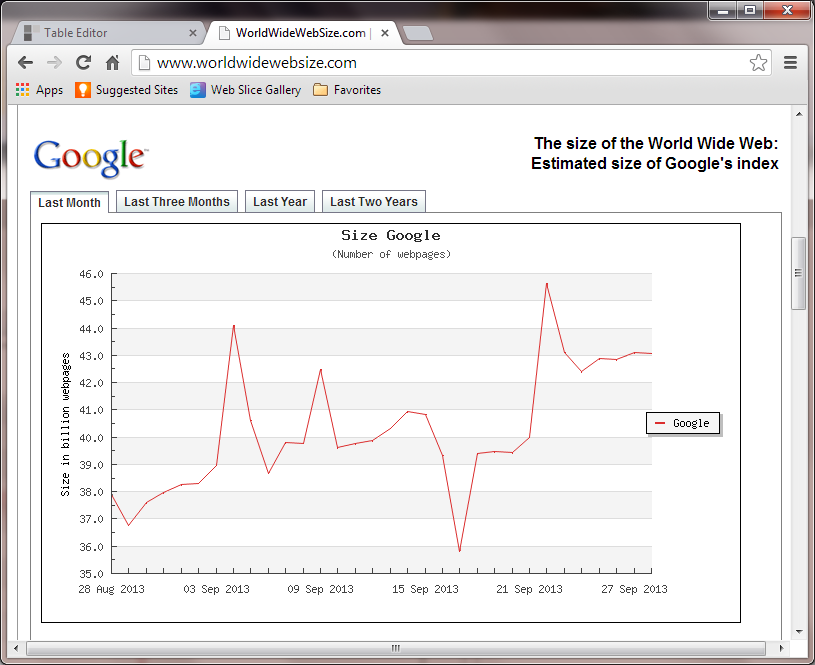
\includegraphics[width=1.00\textwidth]{GoogleEstimatedSize.png}
	\caption{Estimated Size of Google's Index}
	\label{fig:GoogleEstimatedSize}
\end{figure}

\begin{figure}[htbp]
	\centering
		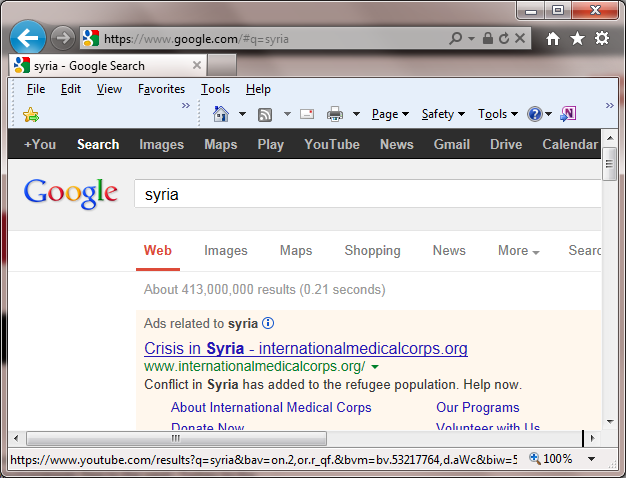
\includegraphics[width=1.00\textwidth]{SyriaQueryHitsGoogle.png}
	\caption{Query Hits for Syria}
	\label{fig:SyriaQueryHitsGoogle}
\end{figure}

\begin{figure}[htbp]
	\centering
		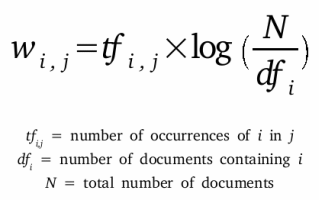
\includegraphics[width=0.50\textwidth]{tfidf.png}
	\caption{TFIDF Equation}
	\label{fig:tfidf}
\end{figure}

\begin{table}
	\centering
    \begin{tabular}{|r|r|r||l|}
    \hline
    TFIDF & TF     & IDF & URI                            \\ \hline
		0.2741 & 0.0409 & 6.7021 & \url{http://beta.syriadeeply.org}           \\ \hline
	  0.1488 & 0.0222 & 6.7021 & \url{http://AmericanSyrians.com}            \\ \hline
    0.1112 & 0.0166 & 6.7021 & \url{http://www.islamicinvitationturkey.com} \\ \hline				
    0.0999 & 0.0149 & 6.7021 & \url{http://www.hhassan.com}                \\ \hline
    0.0838 & 0.0125 & 6.7021 & \url{http://carlsonsperspective.tumblr.com} \\ \hline
    0.0771 & 0.0115 & 6.7021 & \url{http://bigbluerock.wordpress.com}      \\ \hline						
    0.0623 & 0.0093 & 6.7021 & \url{http://www.nationaljournal.com}        \\ \hline
    0.0617 & 0.0092 & 6.7021 & \url{http://brown-moses.blogspot.co.uk}     \\ \hline		
    0.0422 & 0.0063 & 6.7021 & \url{http://goglobalmedia.com}              \\ \hline
    0.0261 & 0.0039 & 6.7021 & \url{http://zamanalwsl.net}                 \\ \hline
    \end{tabular}
    \caption {10 Hits for the term "Syria", ranked by TFIDF}
			\label{tab:TFIDF-Rank}
\end{table}


%%%%%%%%%%Chapter Exercises
\section{Question 3}
\subsection{Problem}Rank the same 10 URIs from question 2, but this time by their PageRank (PR) using any of the free PR estimators on the web. Normalize the returned values to be between 0 and 1.0. Create a table which ranks the URIs by decreasing page rank. Briefly compare and contrast the rankings produced in questions 2 and 3.

\subsection{Response}We submitted each of the URIs to the Google PageRank tool (\url{http://www.checkpagerank.net/}). According to the site, ``Google PageRank (Google PR) is one of the methods Google uses to determine a page's relevance or importance. Important pages receive a higher PageRank and are more likely to appear at the top of the search results.'' The page rank is reported on a scale of 0 to 10 (e.g., 5/10) which we have converted to decimal so the values are between 0 and 1.  Google PR was unable to obtain a ranking for one of the URIs, NA as opposed to 0, which could indicate the site had never been indexed. A representation of the tool is shown in Figure \ref{fig:CheckPageRank}. The final rankings are shown in Table \ref{tab:PageRank}. A comparison of the TFIDF and PageRank outcomes reveals that only one URI, \url{http://goglobalmedia.com}, retained the same position in both lists. This may be more coincidental than a result of any other factors. It is difficult to compare the two methodologies because they are based on different criteria. As stated by Croft \cite{croft2010search}, TFIDF ``reflects the importance of a term in the collection of documents.'' On the other hand, page rank rates poularity based on the number and quality of the links to a particular site.

\begin{figure}[htbp]
	\centering
		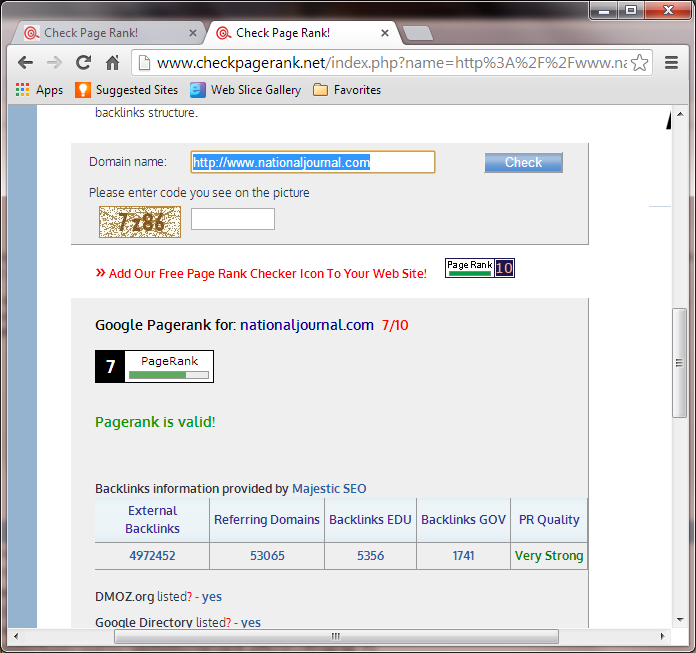
\includegraphics[width=0.60\textwidth]{CheckPageRank.png}
	\caption{Google PR Tool}
	\label{fig:CheckPageRank}
\end{figure}


\begin{table}
	\centering
    \begin{tabular}{|r|l|}
    \hline
    Page Rank & URI                                   \\ \hline
    0.07& \url{http://www.nationaljournal.com}        \\ \hline		
		0.05& \url{http://beta.syriadeeply.org}           \\ \hline
		0.05& \url{http://AmericanSyrians.com}            \\ \hline
    0.04& \url{http://zamanalwsl.net}                 \\ \hline
		0.04& \url{http://brown-moses.blogspot.co.uk}     \\ \hline		
    0.03& \url{http://www.islamicinvitationturkey.com}\\ \hline				
    0.03& \url{http://carlsonsperspective.tumblr.com} \\ \hline
    0.01& \url{http://bigbluerock.wordpress.com}      \\ \hline						
    0.00& \url{http://goglobalmedia.com}              \\ \hline
    NA & \url{http://www.hhassan.com}                 \\ \hline		
    \end{tabular}
    \caption {10 Hits for the term "Syria", ranked by PageRank}
			\label{tab:PageRank}
\end{table}

%%%%%%%%%%Chapter Exercises
\section{Question 4 Extra Credit}
\subsection{Problem}Compute the Kendall Tau\_b score for both lists. Report both the Tau value and the ``p'' value.
\subsection{Response}We used online statistics software to calculate Kendall Tau\_b. The software developed by Wessa\cite{Wessa2012} implements the R Kendall library. For the first input vector, we used the numerical ranking of URIs, by TFIDF, sorted in ascending order. For the second vector, we used the numerical ranking corresponding to the URIs associated page rank. The data source is shown in Table \ref{tab:Kendall}. While the TFIDF rankings were unique, we encountered three ties among the page rank data. The output from the R calculations, Figure \ref{fig:Kendall}, shows a Kendall value of 0.2611 and a p-value of 0.3964. This indicates a 26 percent probability that the two ranking methods will produce the same ordering for the given set of URIs. It's more likely for the rankings to diverge. The p-value represents the confidence interval or statistical significance of tau. Our calculated value is greater than the generally accepted level of 0.05 which seems to strongly suggest that we should not expect similar rankings from TFIDF and Page Rank.

\begin{table}
	\centering
    \begin{tabular}{|r|r|l|}
    \hline
    TFIDF 	& Page Rank     & URI                            \\ \hline
    1				& 5 	& \url{http://zamanalwsl.net}                 \\ \hline
    2				& 1 	& \url{http://goglobalmedia.com}              \\ \hline
    3				& 5 	& \url{http://brown-moses.blogspot.co.uk}     \\ \hline		
    4				& 9 	& \url{http://www.nationaljournal.com}        \\ \hline
    5				& 2 	& \url{http://bigbluerock.wordpress.com}      \\ \hline						
    6				& 3 	& \url{http://carlsonsperspective.tumblr.com} \\ \hline
    7				& NA 	& \url{http://www.hhassan.com}                \\ \hline
    8				& 3 	& \url{http://www.islamicinvitationturkey.com} \\ \hline				
	  9				& 7 	& \url{http://AmericanSyrians.com}            \\ \hline
		10			& 7 	& \url{http://beta.syriadeeply.org}           \\ \hline
    \end{tabular}
    \caption {Kendall Tau\_b Input Vectors}
			\label{tab:Kendall}
\end{table}


\begin{figure}[htbp]
	\centering
		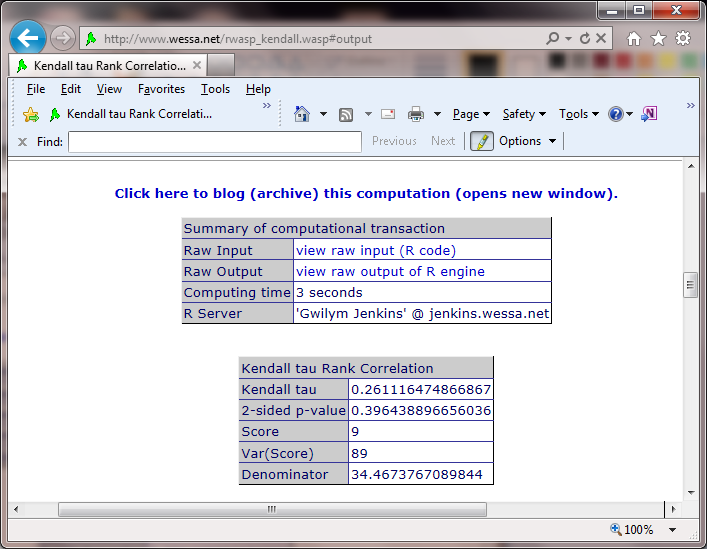
\includegraphics[width=0.70\textwidth]{Kendall.png}
	\caption{Kendall Rank Correlation}
	\label{fig:Kendall}
\end{figure}


\end{savenotes}

% produce the bibliography for the citations in your paper.
\bibliographystyle{abbrv}
\bibliography{cmccoy}

\appendix
\addcontentsline{toc}{chapter}{Appendices}

%%Appendix A
\chapter{Source getHTMLSource Script} \label{chap:getHTML}
\input{getHTMLsource.txt}



\end{document} 
%%%%%%%%%%Ed of report
